% !TEX program = xelatex
% 论文主文档：汇总章节、参考文献与附录。
% 正文内容请到 sections/ 下按章节编辑，避免多人同时改本文件。

\PassOptionsToPackage{quiet}{xeCJK}
\documentclass[withoutpreface,bwprint]{cumcmthesis}

% ================= 宏包与格式 =================
\makeatletter
% 正文五号（10.5pt）；在保证可读性的前提下压缩到约 15pt 基线距
\renewcommand\normalsize{\@setfontsize\normalsize{10.5}{12.0}}
\makeatother
\geometry{top=25mm,bottom=25mm,left=25mm,right=25mm}
\usepackage{etoolbox}
\usepackage{ctex}
\usepackage{graphicx}   % 插图（\includegraphics 必需）
\usepackage{booktabs}   % 三线表（\toprule\midrule\bottomrule）
\usepackage{amsmath}    % 数学公式环境（equation 等）
\BeforeBeginEnvironment{tabular}{\zihao{-5}}
\usepackage[numbers,sort&compress]{natbib}   % 参考文献
\usepackage[framemethod=TikZ]{mdframed}      % 框架
\usepackage{url}
\usepackage{subcaption}                      % 子图

\captionsetup{
    labelfont=bf,
    labelsep=quad,
    format=hang
}
\renewcommand{\captionfont}{\songti\zihao{5}}
\renewcommand{\captionlabelfont}{\bfseries\songti\zihao{5}}

\newcolumntype{C}{>{\centering\arraybackslash}X}
\newcolumntype{R}{>{\raggedleft\arraybackslash}X}
\newcolumntype{L}{>{\raggedright\arraybackslash}X}
\renewcommand{\textbf}[1]{{\song\bfseries #1}}
\AtBeginDocument{%
  \renewcommand{\baselinestretch}{1.25}\normalsize
  \setlength{\abovedisplayskip}{6pt plus 2pt minus 2pt}
  \setlength{\belowdisplayskip}{6pt plus 2pt minus 2pt}
  \setlength{\abovedisplayshortskip}{3pt plus 2pt minus 1pt}
  \setlength{\belowdisplayshortskip}{4pt plus 2pt minus 1pt}
}

% 流程图样式（技术路线图等可用）
\usepackage{tikz}
\usetikzlibrary{calc}
\usetikzlibrary{shapes.geometric, arrows.meta, positioning}
\tikzstyle{startstop}=[rectangle, rounded corners, minimum width=3cm, minimum height=1cm, text centered, draw=black, fill=red!20]
\tikzstyle{process}=[rectangle, minimum width=3.5cm, minimum height=1cm, text centered, draw=black, fill=blue!20]
\tikzstyle{decision}=[diamond, aspect=2, minimum width=3.5cm, minimum height=1cm, text centered, draw=black, fill=green!20]
\tikzstyle{arrow}=[thick,->,>=stealth]

% ================= 论文基本信息 =================
\title{全向与定向干扰源的无源测向定位与自主清除模型}

\begin{document}

\pagenumbering{arabic}   % 电子版摘要为第 1 页，正文连续编号
\maketitle

% 摘要：比赛最后统一定稿，由负责统稿的同学维护。
\begin{abstract}

\textbf{针对问题一：}

\textbf{针对问题二：}

\textbf{针对问题三：}

\textbf{针对问题四：}

\keywords{}

\end{abstract}


% \tableofcontents        % 需要目录时取消注释

% 问题重述与分析
\section{问题重述与分析}

\subsection{问题背景}
无线电频谱的有序使用关系到通信、导航和广播等业务的正常运行。传统干扰排查通常经历初步监测、区域排查和人工近场定位，最后一环耗时且可能使人员暴露于危险环境。搭载测向机、光学定位装置和激光清除装置的四足机器人，能够把这一过程改写为“感知—决策—移动—清除”的自主闭环；但示向误差、未知接收半径、未知频道以及定向源盲区，使系统同时面临几何不确定性和在线路径决策问题\cite{wang2019}。

\subsection{问题重述}
\textbf{问题一：}由若干检测点坐标和同一干扰源的示向度，在 $\pm1^\circ$ 误差下构造交会定位区域，求其直径，并判断以一组直径端点为直径的圆能否覆盖该区域。

\textbf{问题二：}已知某全向干扰源在第一检测点的示向度，设计第二检测点，使再次接收具有确定性保证，并在定位精度与移动检测耗时之间取得权衡，给出候选区域及推荐站址。

\textbf{问题三：}目标圆域内有 $10$--$16$ 个频道互异的全向干扰源，其数量、位置、频道和接收半径均未知；机器狗从原点、频道 1 出发，自主完成发现、定位、清除与不存在认证，并最小化虚拟总时间。

\textbf{问题四：}在问题三中加入数量和朝向均未知的定向干扰源。此时一次无信号还可能由定向盲区造成，需重新设计发现证书与清除策略，并完成模拟器测试。

\subsection{问题分析与总体思路}
四问共享“\textbf{不确定集合—确定性证书—代价最小化}”主线。问题一把每个示向度写成闭凸测向锥，以半平面交获得定位集合，再用凸包与旋转卡壳求直径，并借最小覆盖圆和 Jung 定理回答覆盖性。问题二先由首次正检测构造完整可能源集合，再求保证接收的第二站候选区；以误差盒经 Jacobian 传播所得的最坏位置误差和局部耗时组成 Pareto 双目标，第二次读数返回后仍调用问题一的精确集合与最小覆盖圆作清除判定。

问题三把“存在源的定位清除”和“无源频道的完备认证”同时纳入在线路径：扫描站承担发现与阴性证据积累，多站示向度顺路交会，未达清除证书的频道才补充观测。问题四的关键不再是普通距离覆盖，而是使任意可能源附近的扫描点从各个半平面方向包围该源；只有这种方向完备性成立，连续无信号才足以排除未知朝向的定向源。最终以公开接口的动作日志复核清除闭合性、时间账和几何证书。

% 全文统一的模型假设、题面条件与符号说明
\section{模型假设}

题面已经明确规定的区域尺度、频道数量、动作耗时与设备阈值均作为已知条件使用，
不再列作假设；本文只对题面没有完全刻画、且会影响后续推导的部分作如下统一假设。

\begin{itemize}[itemindent=2em]
  \item \textbf{假设 $1$（静态平面几何）：}一次任务内各干扰源位置保持不变，检测点的平面坐标已知且执行无误差，测向机与干扰源的高度差按题面规定忽略（依据：题面条款与定位必要理想化；用于问题一至问题四）。
  \item \textbf{假设 $2$（目标属性稳定）：}在题面规定的每频道至多一个干扰源的前提下，同一频道的全部有效观测对应同一干扰源，且该源的有效接收半径与定向方向在一局内保持不变（依据：题面条款与任务时段稳定性口径；用于问题一至问题四）。
  \item \textbf{假设 $3$（确定性误差解释）：}不同检测点的示向误差仅满足区间界而不预设独立性或概率分布，同一检测点的固定误差不通过重复检测取平均，所有保证性结论均按误差盒的最坏情形建立（依据：题面条款与最坏情形口径；用于问题一至问题四）。
  \item \textbf{假设 $4$（理想覆盖传播）：}除题面给定的距离衰减、定向覆盖半平面和示向误差外，不再引入额外遮挡、多径或源间干扰，覆盖区内场强只随距离变化（依据：题面条款与模型闭合需要；用于问题一至问题四）。
  \item \textbf{假设 $5$（理想运动控制）：}机器狗视为可即时改变行进方向的质点，指令坐标能够准确到达，除直线移动和题面列明的串行动作耗时外不计转向、加减速及通信计算时间（依据：题面直线运动规则与最短时间建模口径；用于问题二至问题四）。
  \item \textbf{假设 $6$（区域性质与空集处理）：}定位区域按连续闭集处理；半平面交集为空时判为观测不相容或候选构型不可行，不把空集解释为零面积；区域退化为单点或线段时按退化集合定义直径（依据：区域性质与数值稳健性口径；用于问题一至问题四）。
\end{itemize}

\subsection{题面条件与统一口径}

为避免把已知常量误写成假设，四问共同使用的题面条件汇总如下。

\begin{center}
\begin{tabularx}{\textwidth}{L C X}
  \toprule
  条件 & 数值或取值 & 统一解释 \\
  \midrule
  目标圆域半径 & $R_0=1800\ \mathrm{m}$ & 约束干扰源位置，不限制机器狗检测点位于圆域内 \\
  干扰源与频道 & $10\le N_J\le16$，频道编号为 $1$--$20$ & 问题三、四中每频道至多一个源，各源频道互异 \\
  示向误差 & $|e_i|\le\delta=1^\circ$ & 题面保证界，无概率分布；示向度统一按逆时针方位角定义 \\
  有效接收半径 & $1000\le R_j^{\mathrm{recv}}\le1500\ \mathrm{m}$ & 半径不可查询；保证接收按下限，保证超距无信号按上限 \\
  定向覆盖 & 定向方向两侧各 $90^\circ$（含边界） & 几何上表示包含边界的闭半平面，覆盖区内场强与角度无关 \\
  近距离检测 & 距离不超过 $5\ \mathrm{m}$ & 位于有效覆盖区时返回“距离过近”，可直接进入清除 \\
  光学定位与清除 & 距离不超过 $20\ \mathrm{m}$ & 对指定频道的未清除源，成功只取决于距离，与干扰源朝向无关 \\
  运动与检测 & 速度 $5\ \mathrm{m/s}$，检测 $5\ \mathrm{s}$，换频 $1\ \mathrm{s}$ & 换频只由相邻两次合法检测的频道变化触发 \\
  清除耗时 & 成功 $5\ \mathrm{s}$，未发现 $3\ \mathrm{s}$ & \texttt{/clear} 不切换测向机当前频道 \\
  \bottomrule
\end{tabularx}
\end{center}

数学模型使用题面误差界 $\delta=1^\circ$；在线程序另取
$\delta_{\mathrm{num}}=1.01^\circ$，其中增加的 $0.01^\circ$ 只用于吸收示向度两位小数表示和浮点运算的量化余量，
不改变问题一、二的物理误差参数，也不把题面保证值改写为 $1.01^\circ$。
问题一、二只对接口返回正常示向度的观测建模；该响应同时给出
$5<\lVert G-S_i\rVert_2\le R_j^{\mathrm{recv}}\le1500\ \mathrm{m}$，首次正检测还给出
$R_j^{\mathrm{recv}}\ge\max\{1000,\lVert G-S_1\rVert_2\}$，后者用于构造问题二的条件保证接收区。
问题二按题面指定的全向干扰源建立站址模型，不把问题四的定向盲区并入第二检测点可行域。
圆域、闭测向锥及其交集均按闭凸集处理；交集为空或测向 Jacobian 退化时把候选构型判为不可行，
交集退化为单点或线段时则分别按直径为零或线段长度计算。
问题一用正 $720$ 边形内、外逼近目标圆域并同时报告直径下界和上界；在线定位则用外接正 $360$ 边形包围目标圆域，
并用 $128$ 个圆的支撑半平面外包有效接收圆，故用于清除的可行集始终是保守外包围。

数值实现把物理边界向安全侧内缩：保证接收距离采用 $999.99\ \mathrm{m}$，
问题四连续域发现证书采用 $994.99\ \mathrm{m}$，保证超距无信号的程序判据采用 $1500.01\ \mathrm{m}$。

认证清除半径采用 $19.999\ \mathrm{m}$，移动终点的剩余半径采用 $19.998\ \mathrm{m}$，覆盖单元半径采用 $19.5\ \mathrm{m}$；
半平面裁剪的基本距离保护量为 $10^{-6}\ \mathrm{m}$，相同站位判定阈值为 $10^{-7}\ \mathrm{m}$，
最坏测向包围另加 $10^{-3}\ \mathrm{m}$ 外扩量；通用几何比较采用 $10^{-10}$ 的相对容差，矩阵秩判断采用 $10^{-12}$ 的相对阈值，交会角退化判断采用 $10^{-12}$ 的无量纲正弦阈值，这些量均为工程余量而非新的物理参数。

对尚未清除的频道，问题三中的 \texttt{no\_signal} 可能表示“该频道无源”或“超出该源的有效接收半径”；
在条件“该频道确有全向源”下才只剩距离原因。
问题四还增加“检测点位于定向盲区”这一原因，因而只有扫描点的局部凸包证书覆盖整个目标圆域后，
才能把从未获得正检测的频道记为不存在。
若已经发现 $16$ 个异频干扰源，则由源数上界可直接认证其余频道无源；除此以外，
任务完成的程序判据是全部 $20$ 个频道均处于“已清除”或“确认不存在”状态。

程序严格串行调用 \texttt{/enter}、\texttt{/measure}、\texttt{/clear} 与 \texttt{/exit}；
每个新动作使用新的 \texttt{request\_id}，网络故障只以完全相同的请求体和同一标识重试，
因此幂等重试不会增加有效动作或虚拟时间。
题面没有规定 \texttt{/clear} 返回“未发现”的次数上限；问题四在线程序设置每局最多 $5$ 次的工程预算，
预算用尽后转入有误差上界的测向包，或仅在“既有失败圆与当前圆覆盖全部剩余可行域”的末单元证书成立时清除，
所以该预算限制试探代价而不削弱完备性。
程序不读取案例真值，只以四个公开接口的合法响应更新状态。

\section{符号说明}

下表只保留四问正文及统一时间模型所需的符号；“首次出现”指其首次参与实质模型推导的章节。

\begin{center}
\begin{tabularx}{\textwidth}{C X C C}
  \toprule
  符号 & 含义 & 单位或取值 & 首次出现 \\
  \midrule
  $S_i=(x_i,y_i)^{\mathsf T}$ & 第 $i$ 个检测点的位置向量 & $\mathrm{m}$ & 问题一 \\
  $G_j=(x_j,y_j)^{\mathsf T}$ & 第 $j$ 个干扰源的位置向量；单源推导时简写为 $G$ & $\mathrm{m}$ & 问题一 \\
  $\hat\theta_i$ & 第 $i$ 个检测点处测得的示向度 & $[0^\circ,360^\circ)$ & 问题一 \\
  $\theta_i$ & 从检测点 $S_i$ 指向干扰源的真实方位角 & $[0^\circ,360^\circ)$ & 问题一 \\
  $e_i$ & 第 $i$ 次检测的示向误差，$\hat\theta_i=\theta_i+e_i$ & $({}^\circ)$ & 问题一 \\
  $\delta$ & 题面给定的示向误差上界 & $1^\circ$ & 问题一 \\
  $\delta_{\mathrm{num}}$ & 在线定位使用的示向误差半角 & $1.01^\circ$ & 问题三 \\
  $u(\phi)$ & 方位角 $\phi$ 对应的二维单位方向向量 & 无量纲 & 问题一 \\
  $W_i$ & 第 $i$ 次示向度对应的闭凸测向锥 & 集合 & 问题一 \\
  $K,\ K_q^-,\ K_q^+$ & 精确定位区域及其内接、外接正 $q$ 边形逼近 & 集合 & 问题一 \\
  $q$ & 目标圆域离散逼近的正多边形边数 & $720$ & 问题一 \\
  $D(K)$ & 定位区域内任意两点距离的最大值 & $\mathrm{m}$ & 问题一 \\
  $r_{\mathrm{MEC}}(K)$ & 定位区域最小覆盖圆的半径 & $\mathrm{m}$ & 问题一 \\
  \bottomrule
\end{tabularx}
\end{center}

\begin{center}
\begin{tabularx}{\textwidth}{C X C C}
  \toprule
  符号 & 含义 & 单位或取值 & 首次出现 \\
  \midrule
  $R_0$ & 目标圆域半径 & $1800\ \mathrm{m}$ & 问题一 \\
  $R_j^{\mathrm{recv}}$ & 第 $j$ 个干扰源的有效接收半径 & $[1000,1500]\ \mathrm{m}$ & 问题二 \\
  $U_1$ & 第一次正常示向度给出的完整可能源集合 & 集合 & 问题二 \\
  $X,\ S_2$ & 第二检测点候选位置与最终选定位置 & $\mathrm{m}$ & 问题二 \\
  $\mathcal C_{1000},\ \mathcal C_{\mathrm{det}}$ & 保守保证接收区与利用首次正检测信息的条件保证区 & 集合 & 问题二 \\
  $J$ & 测向模型对干扰源位置的 Jacobian 矩阵 & $\mathrm{rad/m}$ & 问题二 \\
  $K_{\mathrm{LS}}$ & 测角残差到位置增量的最小二乘增益矩阵 & $\mathrm{m/rad}$ & 问题二 \\
  $\Sigma_G$ & 一阶位置估计协方差矩阵 & $\mathrm{m^2}$ & 问题二 \\
  $\gamma$ & 两条交会视线的锐夹角 & $[0^\circ,90^\circ]$ & 问题二 \\
  $\mathrm{GDOP}$ & 测向几何精度衰减因子 & $\mathrm{m/rad}$ & 问题二 \\
  $f_1(X),\ f_2(X)$ & 确定性最坏位置误差与第二次检测耗时 & $\mathrm{m},\ \mathrm{s}$ & 问题二 \\
  $\mathcal P$ & 精度与耗时的 Pareto 非支配候选点集 & 集合 & 问题二 \\
  \bottomrule
\end{tabularx}
\end{center}

\begin{center}
\begin{tabularx}{\textwidth}{C X C C}
  \toprule
  符号 & 含义 & 单位或取值 & 首次出现 \\
  \midrule
  $P_k$ & 第 $k$ 个扫描点或路径节点的位置 & $\mathrm{m}$ & 问题三 \\
  $N_J$ & 一局中的干扰源总数 & $10,\ldots,16$ & 问题三 \\
  $N_m,N_s$ & 检测次数与换频次数 & 次 & 问题三 \\
  $N_c^{\mathrm{succ}},N_c^{\mathrm{miss}}$ & 成功清除与未发现清除的次数 & 次 & 问题三 \\
  $T$ & 定位清除任务的虚拟总时间 & $\mathrm{s}$ & 问题三 \\
  $V_G$ & 距可能源位置 $G$ 不超过 $1000\ \mathrm{m}$ 的扫描点相对向量集 & 集合 & 问题四 \\
  $d$ & 定向干扰源的单位发射方向向量 & 无量纲 & 问题四 \\
  $P_4,\ P_4'$ & 问题四的基准扫描点集与连续域认证提速点集 & 集合 & 问题四 \\
  \bottomrule
\end{tabularx}
\end{center}

\begin{table}[H]
\centering
\begin{minipage}[t]{0.9\textwidth}
\centering
\caption{术语与状态表}
\small
\begin{tabular}{@{}p{3.4cm}p{9.6cm}@{}}
\toprule
术语 & 含义（单位） \\
\midrule
MEC & 最小覆盖圆 (Minimum Enclosing Circle) \\
GDOP & 几何精度衰减因子 $\sqrt{\operatorname{tr}[(H^{\mathsf T}H)^{-1}]}$ (m/rad) \\
RMS & 一阶位置均方根误差 (m) \\
Pareto 前沿 & 两目标下不被其他可行解支配的候选点集 (集合) \\
\texttt{unknown} & 尚未发现该频道源 (状态枚举) \\
\texttt{positively\_detected} & 该频道至少得到一次正常示向度或“距离过近” (状态枚举) \\
\texttt{localizing} & 正在追加异地观测并收缩定位区域 (状态枚举) \\
\texttt{clear\_ready} & 外近似 MEC 半径不超过 20 m，或返回“距离过近” (状态枚举) \\
\texttt{cleared} & 该频道干扰源已成功清除 (状态枚举) \\
\texttt{absent\_certified} & 保证扫描全部完成且该频道从未被正检测 (状态枚举) \\
\texttt{geometry\_fault} & 保证分支失信号、空交集或认证清除失败 (阻断状态) \\
\texttt{clear\_fallback} & 对当前外近似执行有限 20 m 覆盖清除 (状态枚举) \\
\texttt{request\_id} & 单次测试会话内的 HTTP 幂等键 (字符串) \\
虚拟时间 & 模拟器按移动与动作规则累计的任务耗时 (s) \\
现实截止时刻 & \texttt{/enter} 返回的剩余程序运行时间约束 (s) \\
\bottomrule
\end{tabular}
\end{minipage}
\end{table}

\section{问题分析}

\textbf{问题一：}此问要求根据检测点坐标和示向度确定定位区域并求其直径，进而判断直径圆能否覆盖该区域。由于测向误差不超过 \(1^\circ\)，不能将示向度视为精确射线，而应把真实方位角视为落在以测得方向为中心、张角 \(2^\circ\) 的扇形内。因此，每个检测点给出一个凸锥约束，干扰源必须位于所有凸锥的交集内。同时，干扰源还受限于半径 \(1800\,\mathrm{m}\) 的目标圆域，故定位区域为多个凸锥与圆域的交集。若交集为空，说明观测不相容；若退化为点或线段，则按退化情形处理。求解时，可将圆域用多边形逼近，把问题转化为半平面求交，得到凸多边形定位区域，再利用凸性求其直径。最后，针对直径圆能否覆盖区域，需分析区域形状，并考虑反例与最小覆盖圆的关系。整体思路是：误差建模 \(\to\) 凸锥交会 \(\to\) 圆域约束 \(\to\) 多边形逼近 \(\to\) 直径计算 \(\to\) 覆盖性讨论。

\textbf{问题二：}此问基于第一问覆盖问题的求解，考虑第一次检测点 \(S_1\) 及示向度 \(\hat\theta_1\) 已知，而第二次检测点 \(S_2\) 待设计的情况。第一次观测给出带误差的示向锥，结合目标距离大于 \(5\mathrm{m}\)、接收半径不超过 \(1500\mathrm{m}\) 及目标圆域，得可能源集合 \(U_1\)。第二检测点须先保证能再次收到信号：最保守取到 \(U_1\) 任意点距离不超过 \(1000\mathrm{m}\) 的核心保证区 \(\mathcal C_{1000}\)；利用第一次成功接收提供的距离信息，可放宽为条件保证区 \(\mathcal C_{\det}\)。精度目标是两次交会后定位区域面积最小，但第二次示向度未知且面积非凸，故采用一阶误差传播构造面积代理 \(A_{\mathrm{cert}}=\pi F_1^2\)，选点后再用问题一模型计算实际区域与最小覆盖圆。按“\(U_1\)—候选区—面积代理—Pareto 选点—数值验证”展开，最终给出第二检测点可行分布与推荐策略。接收可靠是首要约束，不能只追求交会角接近直角。

\textbf{问题三：}此问在前面两问研究的基础上，要求机器狗从原点出发、初始频道为 1，在 10–16 个全向干扰源数量未知、频道未知、位置未知、有效接收半径未知的条件下，完成全部干扰源的定位与清除，并使总时间尽可能短。与问题一、二相比，本问的核心困难有三点：1.发现性：没有任何先验位置信息，必须设计一套有限步内必能发现全部干扰源的扫描方案，并且要能对"某频道不存在"给出结论，否则无法判断任务是否真正完成。
2.定位的收敛性：每次测向只给出 $1^\circ$ 的角度信息，单次交会无法直接达到光学清除所需的精度，需要设计保证能持续获得新观测的取点规则。
3.计时口径：总时间包含移动、换频、检测、光学精确定位与清除，各项耗时规则不同（移动按距离除以 5 m/s，换频 1 s，检测 5 s，清除成功 5 s、未发现 3 s），策略必须与实际计时规则一一对应。

\textbf{问题四：}此问在问题三的基础上，新增要求：目标区域内除全向干扰源外还存在定向干扰源，其个数与定向方向均未知。这一差别改变了问题的一个基本逻辑，即问题三中"某个频道扫不到信号"只有两种解释：该频道没有干扰源，或距离超过有效接收半径，两者都能由扫描覆盖证书排除，所以"扫描点全部测完仍无信号"可以作为"该频道不存在"的证明。而问题四中多出第三种解释：检测点位于该定向干扰源的盲区。定向干扰源的有效覆盖角为定向方向两侧各 $90^\circ$，覆盖角之外没有信号辐射。为解决新增情况带来的判断问题，先设计对任意未知朝向都保证发现的扫描骨架。固定可能源位置 \(G\)，记其接收半径内扫描点为 \(V_G\)。若全部扫描点均不可见，则存在方向使所有 \(P_j-G\) 落在同一开半平面内，等价于 \(0\notin\operatorname{conv}V_G\)。故只要保证
\[
G\in\operatorname{conv}\{P_j:\|P_j-G\|\le1000\},\quad \forall G\in B_{1800},
\]
就能对任意朝向至少有一个扫描点可见。据此可取边长 \(990\,\mathrm{m}\) 的等边三角格，扫描其与目标圆域相交的基本三角形顶点，共 \(31\) 点；或用 \(22\) 点认证集配合连续域凸包证书提速。
同时在定位与清除上，首个示向度仍给出位置扇形，但首点可能位于盲区边界，后续 \texttt{no\_signal} 不再视为故障，而是触发完备路径：在扇形上铺 \(20\,\mathrm{m}\) 三角格逐点清除，有限步内必清除成功；一旦新增观测使最小覆盖圆半径降到 \(20\,\mathrm{m}\) 内，则回到单点清除。状态转移与问题三基本相同，但“确认不存在”必须满足上述凸包条件。

\subsection{总体框架}

%问题一
\section{问题一的模型建立与求解}

\subsection{模型准备}

\subsection{模型建立}

\subsection{模型求解与结果分析}

\subsection{小结}
% 问题二
\section{问题二的模型建立与求解}

\subsection{模型准备}

\subsection{模型建立}

\subsection{模型求解与结果分析}

\subsection{小结}
% 问题三
\section{问题三的模型建立与求解}

\subsection{模型准备}

\subsubsection{动作协议与时间模型}

机器狗的位置和当前频道由相邻动作的位置、频道参数唯一确定，求解过程只需维护该状态。为避免网络重试重复计入，重试沿用原 \texttt{request\_id} 与载荷，并同时校验 HTTP 状态和响应中的 \texttt{accepted} 字段；在线算法记录剩余现实时间并保留截止余量。

\subsubsection{几何证据与清除证书}

对频道 $c$ 在测站 $S$ 的一次测量结果作如下解释：

\begin{enumerate}
\item \texttt{direction}：返回正常示向度 $\hat\theta_c(S)$，用于生成示向锥；
\item \texttt{near}：测站与目标的距离不超过 $5\mathrm{m}$，可直接在测站清除；
\item \texttt{no\_signal}：当前测站不在该源的有效接收范围内，只能作为阴性证据，不能单独证明频道为空。
\end{enumerate}

频道 $c$ 的可行定位区域记为 $K_c$。在线算法以多边形外包围 $A_c$ 代替精确圆弧边界，并保持

\begin{equation}
K_c\subseteq A_c.
\label{eq:q3_outer_contain}
\end{equation}

利用问题一的半平面裁剪算法更新 $A_c$\cite{sutherland1974}。设 $C_c$ 为 $A_c$ 的覆盖圆心，定义保守半径

\begin{equation}
\rho_c=\max_{X\in A_c}\lVert X-C_c\rVert_2.
\label{eq:q3_outer_radius}
\end{equation}

由于欧氏范数是凸函数，其在凸多边形上的最大值必在顶点取得。若

\begin{equation}
\rho_c\le r_{\mathrm{opt}}-\epsilon_{\mathrm{num}},
\qquad
\epsilon_{\mathrm{num}}=0.001\mathrm{m},
\label{eq:q3_clear_certificate}
\end{equation}

则任取 $G\in K_c$，均有 $\lVert G-C_c\rVert_2\le\rho_c<20\mathrm{m}$，故在 $C_c$ 处执行的清除动作具有严格几何证书。若为衔接路径而偏移清除点，则仅当该点到 $A_c$ 全部顶点的最远距离仍不超过 $19.999\mathrm{m}$ 时执行；由 $K_c\subseteq A_c$，此时对真实源的距离证书仍然成立。若检测结果直接为 \texttt{near}，则在当前测站清除。除这两种情形外，不执行试探性清除。

\subsubsection{频道状态与终止条件}

每个频道维护一个状态，其含义如表~\ref{tab:q3_states}所示。

\begin{table}[htbp]
\centering
\small
\setlength{\tabcolsep}{3pt}
\caption{问题三频道状态及进入条件}
\label{tab:q3_states}
\begin{tabularx}{\textwidth}{@{}p{0.20\textwidth}p{0.28\textwidth}X@{}}
\toprule
状态 & 含义 & 进入条件 \\
\midrule
\texttt{unknown} & 尚未发现目标，也尚未认证为空 & 初始状态 \\
\texttt{localizing} & 已发现目标，正在收缩定位区域 & 已获得正常示向度，但尚未达到清除条件 \\
\texttt{clear\_ready} & 当前外包围已满足光学清除半径 & $\rho_c\le19.999\mathrm{m}$ \\
\texttt{cleared} & 已成功清除 & \texttt{/clear} 返回成功 \\
\texttt{absent\_certified} & 已证明频道内不存在干扰源 & 七站均实测无信号或已有严格推断，或已发现 16 源 \\
\texttt{geometry\_fault} & 定位区域为空或认证后的动作无法闭合证书 & 空区域、认证清除失败或有限覆盖仍未闭合等异常 \\
\bottomrule
\end{tabularx}
\end{table}

终止判据要求，仅当所有频道均已清除或认证为空时，才可调用一次 \texttt{/exit}。若仍存在未发现频道、定位未闭合频道或几何故障状态，则任务尚未闭合，不能报告为完成。

\subsection{模型建立}

\subsubsection{七点扫描覆盖与发现证书}

取

\begin{equation}
P_0=(0,0),
\qquad
P_k=1200\left(\cos\frac{k\pi}{3},\ \sin\frac{k\pi}{3}\right),
\quad k=1,\ldots,6.
\label{eq:q3_scan_sites}
\end{equation}

七点集合记为 $\mathcal S$。将目标圆域按六个 $60^\circ$ 扇区划分，第 $k$ 个扇区以 $P_k$ 为中心方向。对扇区内任一点 $G$，记 $r=\lVert G\rVert_2$，其相对 $P_k$ 的夹角为 $\varphi\in[-30^\circ,30^\circ]$。由于构型关于每个扇区的中线对称，只需分析 $0\le\varphi\le30^\circ$；六个扇区除旋转外完全相同。

原点与 $P_k$ 到 $G$ 的距离相等当且仅当

\begin{equation}
r=\frac{600}{\cos\varphi}.
\label{eq:q3_voronoi_boundary}
\end{equation}

若 $r\le600/\cos\varphi$，则到原点的距离不超过

\begin{equation}
\frac{600}{\cos30^\circ}=400\sqrt3\approx692.82\mathrm{m}.
\label{eq:q3_inner_bound}
\end{equation}

若 $r\ge600/\cos\varphi$，则到 $P_k$ 的平方距离关于 $r$ 是凸二次函数，其在区间 $[600/\cos\varphi,1800]$ 的端点取得最大值。径向左端点处两扫描点到 $G$ 的距离相等且不超过 $692.82\mathrm{m}$；目标圆域外端点对应的距离为

\begin{equation}
f(\varphi)
=
\sqrt{1800^2+1200^2-2\cdot1800\cdot1200\cos\varphi}.
\label{eq:q3_outer_radial}
\end{equation}

$f(\varphi)$ 在 $0\le\varphi\le30^\circ$ 上单调增加，故

\begin{equation}
d_{\max}
=f(30^\circ)
=
\sqrt{1800^2+1200^2-2\cdot1800\cdot1200\cos30^\circ}
=968.9015717\mathrm{m}.
\label{eq:q3_dmax}
\end{equation}

因此，目标圆域内任一点到 $\mathcal S$ 中最近扫描点的距离不超过 $d_{\max}$；图~\ref{fig:q3_scan_certificate}给出了扫描点、接收圆盘与最坏边界位置的关系。

\begin{figure}[htbp]
\centering
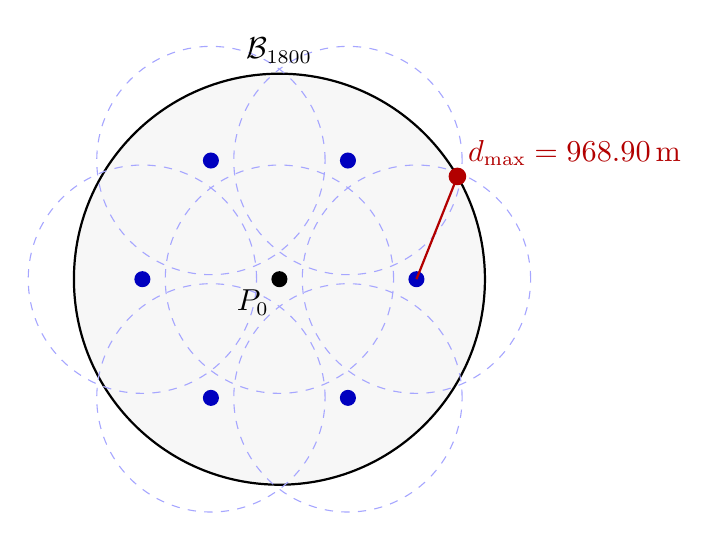
\begin{tikzpicture}[scale=1.45]
  \fill[black!3] (0,0) circle (1.8);
  \draw[thick] (0,0) circle (1.8);
  \draw[blue!35,dashed] (0,0) circle (1.0);
  \fill[black] (0,0) circle (2pt);
  \foreach \k in {0,...,5}{
    \coordinate (Q\k) at ({1.2*cos(60*\k)},{1.2*sin(60*\k)});
    \draw[blue!35,dashed] (Q\k) circle (1.0);
    \fill[blue!75!black] (Q\k) circle (2pt);
  }
  \coordinate (W) at ({1.8*cos(30)},{1.8*sin(30)});
  \fill[red!70!black] (W) circle (2.2pt);
  \draw[red!70!black,thick] (Q0)--(W);
  \node[above] at (0,1.8) {$\mathcal B_{1800}$};
  \node[below left] at (0,0) {$P_0$};
  \node[above right,red!70!black] at (W) {$d_{\max}=968.90\,\mathrm m$};
\end{tikzpicture}
\caption{问题三七点扫描骨架、接收覆盖与最坏位置}
\label{fig:q3_scan_certificate}
\end{figure}

\textbf{命题 1（发现完备性）}　若 $1000\mathrm{m}\le r_j^{\mathrm{recv}}\le1500\mathrm{m}$，则每个干扰源在七个扫描点中至少一个点上会被检测到；若某频道在七个扫描点上均返回 \texttt{no\_signal}，则该频道必不存在干扰源。

证明：由 $d_{\max}<1000\mathrm{m}$，任一干扰源到最近扫描点的距离不超过 $968.9016\mathrm{m}$，位于其有效接收范围内。由于问题三中的干扰源为全向源，该点不会出现方向盲区，因此测量结果只能是 \texttt{direction} 或 \texttt{near}。反之，若七个点均无信号，则与上述必然有信号矛盾。证毕。

七个扫描点构成发现证书，其正确性只依赖扫描点的集合，与访问顺序无关。因此，后续为缩短路径而重排扫描站不会削弱该证书。

若某频道已经获得一次有效响应，则记为“已发现源”；同一频道的多次观测只对应一个源。当已发现不同频道数达到 16 时，根据干扰源总数不超过 16 以及频道唯一性，剩余频道必为空，可直接认证为 \texttt{absent\_certified}。该结论可缩短扫描过程，且不需要额外的阴性观测。

\subsubsection{阴性证据推理}

设 $Q$ 是频道 $c$ 的一个无信号站，$S$ 是尚未测量但可接收该源的候选站，并记该源的有效接收半径为 $r^{\mathrm{recv}}$。若目标 $G$ 在 $S$ 处可接收而在 $Q$ 处不可接收，则

\begin{equation}
\lVert G-S\rVert_2\le r^{\mathrm{recv}}<\lVert G-Q\rVert_2.
\label{eq:q3_negative_order}
\end{equation}

平方后可得

\begin{equation}
(Q-S)^{\mathsf T}G
<
\frac{\lVert Q\rVert_2^2-\lVert S\rVert_2^2}{2}.
\label{eq:q3_negative_halfplane}
\end{equation}

右端等于 $(Q-S)^{\mathsf T}(Q+S)/2$，因此上式定义一个开半平面。将其与目标圆域、距离上界以及其余无信号站产生的不等式求交，若交集为空，则候选站 $S$ 不可能接收该源，扫描时可直接跳过并记为推断无信号。

另一种阴性证据来自圆盘覆盖：设候选区域被若干已测得无信号站周围半径 $1000\mathrm{m}$ 的圆盘覆盖。若源位于该区域，则它到某个无信号站的距离不超过 $1000\mathrm{m}\le r^{\mathrm{recv}}$，该站本应收到信号，与事实矛盾。因此，只要连续区域的圆盘覆盖关系成立，即可安全跳过相应测量。推断阴性只用于更新认证状态，不记录为实际测量结果。

\subsubsection{保证有信号的第二测站}

设首次正常示向度为 $\hat\theta$，其单位方向为 $d=d(\hat\theta)$，左法向量为 $d^{\perp}=d^{\perp}(\hat\theta)$。取

\begin{equation}
S'=S+400d+300d^{\perp}.
\label{eq:q3_safe_site}
\end{equation}

该点与首点的距离为 $500\mathrm{m}$，相对首条视线的横向偏移为 $300\mathrm{m}$。

设首点测得方向时源距为 $r$，真实方向与名义方向的夹角为 $\varepsilon_\theta$，满足 $|\varepsilon_\theta|\le\delta_{\mathrm{num}}$。位移向量 $w=S'-S=400d+300d^{\perp}$，令 $a=w\cdot d(\hat\theta+\varepsilon_\theta)$，则

\begin{equation}
a
=400\cos\varepsilon_\theta+300\sin\varepsilon_\theta
\ge400\cos\delta_{\mathrm{num}}-300\sin\delta_{\mathrm{num}}
>394.6\mathrm{m}.
\label{eq:q3_projection_bound}
\end{equation}

因此

\begin{equation}
\begin{aligned}
\lVert G-S'\rVert_2^2
&=r^2+500^2-2ra\triangleq\Phi(r).
\end{aligned}
\label{eq:q3_distance_change}
\end{equation}

$\Phi(r)$ 是开口向上的二次函数。若 $r\ge1000\mathrm{m}$，则由 $a>394.6\mathrm{m}$ 得 $250000-2ar<0$，故 $\lVert G-S'\rVert_2<r\le r^{\mathrm{recv}}$。若 $r<1000\mathrm{m}$，则 $\Phi$ 在 $[0,1000]$ 上的最大值必在端点取得，而
\[
\Phi(0)=500^2<1000^2,
\qquad
\Phi(1000)=1000^2+500^2-2000a<1000^2.
\]
因此 $\lVert G-S'\rVert_2<1000\mathrm{m}\le r^{\mathrm{recv}}$。综上，$S'$ 必能收到该源的有效响应。该构造只改变测量位置，不增加误差分布假设。

\subsubsection{定位区域更新与测站选择}

初始化频道 $c$ 的外包围为覆盖目标圆域的正多边形。获得正常示向度后，依次执行：

\begin{enumerate}
\item 用 $\delta_{\mathrm{num}}$ 生成示向锥 $W(S,\hat\theta_c)$ 的两条半平面；
\item 与外包围 $A_c$ 求交；
\item 用 $\lVert G-S\rVert_2\le1500\mathrm{m}$ 的圆域支撑半平面继续裁剪；
\item 对每个无信号站 $Q\in\mathcal D_c$，用半平面 $R(Q,S)$ 排除不可能位置；
\item 重新计算外包围的覆盖圆心 $C_c$ 和保守半径 $\rho_c$。
\end{enumerate}

若 $A_c$ 为空，则报告观测矛盾；若 $\rho_c\le19.999\mathrm{m}$，则转入清除；否则继续选择新测站。正常测站候选满足以下条件：

\begin{enumerate}
\item 具有接收保证：候选点到当前外包围中任一点的距离均小于 $999.99\mathrm{m}$，对应数学上的严格接收保证，并保留 $0.01\mathrm{m}$ 的数值余量；或候选点到该外包围中每一点的距离都严格小于某个既有成功观测站到相应点的距离，从而利用首次成功接收所给出的接收半径下界；
\item 候选点到当前外包围的最远距离不超过 $1499.99\mathrm{m}$，从而除非目标距候选点不超过 $5\mathrm{m}$ 并转入 \texttt{near} 清除，否则返回的方向必为有效 \texttt{direction}；
\item 名义方位预评估显示其能使定位半径下降；
\item 当 $\rho_c\le450\mathrm{m}$ 时，对可能返回的方位按不超过 $2^\circ$ 分箱，并对每个分箱扩大误差半角后计算裁剪区域半径上界；优先选择上界不超过 $19.5\mathrm{m}$ 或小于当前半径 $75\%$ 的测站。若不存在这样的改进候选，则回到基础候选规则，不把启发式上界误当成可行性硬约束。
\end{enumerate}

最后一项使用误差上界而非名义方位做决策，避免因未知返回值导致测站选择乐观失效。所有候选步骤仍以问题一的半平面交和最小覆盖圆为几何内核。

当 $\rho_c\le300\mathrm{m}$ 时，采用十二点环形测站包：

\begin{equation}
a_c=1.2\rho_c+8,
\qquad
S_i=C_c+a_c\left(\cos\psi_i,\sin\psi_i\right),
\quad
\psi_i=\psi_0+\frac{i\pi}{6}.
\label{eq:q3_packet_sites}
\end{equation}

任一测站到可能源的距离不超过

\begin{equation}
a_c+\rho_c=2.2\rho_c+8\le668\mathrm{m},
\label{eq:q3_packet_receive}
\end{equation}

故十二个测站均有信号保证。十二个方位均匀分布的测站用于改善交会几何，是否继续访问仍由保守半径的实际收缩判定。每轮最多访问十二个环点；一旦半径降至本轮初始值的 $55\%$ 以下或达到清除阈值，本轮提前结束。外层在 $\rho_c\le300\mathrm{m}$ 时最多重复 8 轮，每轮均按更新后的 $C_c$ 和 $\rho_c$ 重建测站包；若仍不足以达到清除阈值，则转入有限覆盖兜底。

\subsubsection{有限覆盖清除与完备性}

当快速定位分支停滞时，对当前外包围 $A_c$ 进行递归细分。每次沿投影跨度较大的方向将单元二分，直到每个叶单元的保守半径不超过

\begin{equation}
\varepsilon_{\mathrm{cov}}=4.5\mathrm{m}.
\label{eq:q3_cover_radius}
\end{equation}

对单元中心 $S$ 执行一次检测。若真实源位于该单元，则

\begin{equation}
\lVert G-S\rVert_2\le\varepsilon_{\mathrm{cov}}<5\mathrm{m},
\label{eq:q3_near_guarantee}
\end{equation}

测量结果必为 \texttt{near}，随后在该点执行光学清除。保证测站若返回 \texttt{no\_signal}，说明该观测与接收保证证书冲突；算法不会将任务直接判为成功，而是结束当前快速分支并进入本有限覆盖过程。只有有限覆盖完成后仍未取得合法清除证书时，才报告几何故障。

覆盖细分只保留与当前外包围仍有交集的单元，而真实源始终属于当前外包围，因此真实源所在叶单元不会被丢弃。单元半径按全部顶点到覆盖圆心的最大距离保守计算；每次对当前较大投影跨度作二分，随着单元尺寸收缩，有限步内即可达到 $4.5\mathrm{m}$。该分支不依赖空清除；若数值退化导致单元覆盖无法推进，算法报告几何故障，而不是假定清除成功。

综上，在本章假设下，每个实际存在的全向干扰源都能被发现并最终获得合法清除路径；每个未发现频道也都有实测 \texttt{no\_signal}、严格阴性推断或 16 源上界之一作为认证依据。因此，终止时不会出现未闭合频道。

\subsubsection{联合路径调度模型}

在时间表达式中，单次检测、换频和清除的时间固定，主要可控项为总移动距离 $L$。设当前重规划时刻的必选任务节点集为

\begin{equation}
V_t=V_t^{\mathrm{scan}}\cup V_t^{\mathrm{service}},
\label{eq:q3_task_nodes}
\end{equation}

其中 $V_t^{\mathrm{scan}}$ 为尚未完成必要阴性认证的扫描站，$V_t^{\mathrm{service}}$ 为已完成发现但仍需定位或清除的频道服务点。后者以该频道当前的保守覆盖圆心 $C_c$ 作为规划位置。对由 $n_t$ 个节点组成的访问顺序 $\sigma=(\sigma_1,\ldots,\sigma_{n_t})$，开放路径长度定义为

\begin{equation}
L(\sigma)
=
\lVert P_{\sigma_1}-P_{\mathrm{cur}}\rVert_2
+
\sum_{i=1}^{n_t-1}
\lVert P_{\sigma_{i+1}}-P_{\sigma_i}\rVert_2,
\label{eq:q3_open_path}
\end{equation}

其中 $P_{\mathrm{cur}}$ 为当前机器狗位置，开放路径不要求返回起点。当前节点集上的调度子问题为

\begin{equation}
\min_{\sigma}\quad L(\sigma).
\label{eq:q3_route_problem}
\end{equation}

节点数不超过 10 时，采用 Held--Karp 动态规划求精确开放路径。令 $d_{ij}$ 为节点间距离，状态 $F_{\mathrm{path}}(M,j)$ 表示从当前点出发访问集合 $M$ 且最后位于 $j$ 的最短距离，则

\begin{equation}
F_{\mathrm{path}}(M,j)
=
\min_{i\in M\setminus\{j\}}
\left[
F_{\mathrm{path}}(M\setminus\{j\},i)+d_{ij}
\right],
\qquad
F_{\mathrm{path}}(\{j\},j)=d_{\mathrm{cur},j}.
\label{eq:q3_held_karp}
\end{equation}

节点数超过 10 时，计算量显著上升，故先以最小增量插入构造初始解，并加入 3 个最近邻起点，再交替执行 2-opt 逆向交换和 Or-opt 邻域重定位直至无改善。此时只声称得到高质量可行路径，不声称是全局最优解。

在每个扫描站内部，除必需的未知频道外，还可在联合调度预测成本较低的条件下，顺势补测已发现且尚未达到清除精度的频道。仅当预期定位半径明显下降，且预计节省的往返时间超过本次测量与换频成本时，才将该测量加入站内任务；否则留给后续必经站处理。该“顺路收获”不改变动作次数的下限，但可减少为同一频道多次往返。

每完成一个联合路径节点（一次扫描站访问或一个频道的服务过程）后，在线算法重新更新频道状态、删除已闭合的扫描站或服务点，并再次求解当前节点集上的开放路径。动态重规划使后续路径能够利用新增方位和清除结果，但不改变七点发现证书。

\subsubsection{算法流程}

上述证书与动态调度合并为下面的在线闭环。伪代码只调用前文已经定义的几何算子；其中
$\operatorname{Update}_3$ 按响应分别执行示向锥裁剪、阴性证据更新或近距清除，
$\operatorname{Certify}_3$ 仅依据完整七点证书或已发现 16 个异频源关闭未知频道。

\begin{mdframed}[
  nobreak=true,
  linewidth=0.6pt,
  innerleftmargin=7pt,
  innerrightmargin=7pt,
  innertopmargin=5pt,
  innerbottommargin=2pt,
  skipabove=6pt,
  skipbelow=6pt
]
\textbf{算法 1\quad 问题三证书驱动联合调度}
\begin{tabbing}
00\quad\=\quad\quad\=\quad\quad\=\kill
1 \> 构造七点扫描集，调用一次 \texttt{/enter}；初始化频道轨迹 $T_c$、$U\leftarrow\mathcal S$、$P\leftarrow O$；\\
2 \> \textbf{while} 存在未闭合频道 \textbf{do}\\
3 \>\> $\operatorname{Certify}_3(T,U)$，并用阴性圆盘覆盖推断可安全退役的扫描站；\\
4 \>\> $V\leftarrow V^{\rm scan}(U)\cup V^{\rm service}(T)$，$a\leftarrow\operatorname{First}(\operatorname{JointRoute}(P,V))$；\\
5 \>\> \textbf{if} $a$ 不存在 \textbf{then break}；\\
6 \>\> \textbf{if} $a$ 为扫描站 $S_i$ \textbf{then}\\
7 \>\>\> $U\leftarrow U\setminus\{S_i\}$，按“必测频道 $\cup$ 有严格净收益频道”的顺序检测；\\
8 \>\>\> 对每个响应 $y$ 执行 $\operatorname{Update}_3(T_c,S_i,y)$，随后重新认证频道；\\
9 \>\> \textbf{else}\quad 令 $c$ 为服务频道，在保证接收的候选点中最小化移动与误差代价；\\
10\>\>\> 最多自适应检测 10 次；若连续两次收缩不足或返回无信号，则停止该层；\\
11\>\>\> 若 $\rho_c\le300\,\mathrm m$ 仍未闭合，则至多执行 8 轮 12 点测站包；\\
12\>\>\> 若 $\rho_c\le19.999\,\mathrm m$，在通过顶点距离证书的位置调用 \texttt{/clear}；\\
13\>\>\> 否则将 $A_c$ 细分为半径不超过 $4.5\,\mathrm m$ 的单元，逐中心检测至近距或半径证书清除；\\
14\>\> \textbf{end if}；若兜底耗尽仍未闭合，则置为 \texttt{geometry\_fault} 并停止；\\
15\> \textbf{end while}；核验 20 个频道均为 \texttt{cleared} 或 \texttt{absent\_certified}；\\
16\> 核验清除数属于 $[10,16]$，仅调用一次 \texttt{/exit}。
\end{tabbing}
\end{mdframed}

\subsection{模型求解与结果分析}

\subsubsection{计算参数}

在线计算采用 $\delta_{\mathrm{num}}=1.01^\circ$ 作为安全半角。目标圆域初始外包围采用 360 条支撑半平面，距离圆域采用 128 条支撑半平面，清除半径使用 $19.999\mathrm{m}$ 的保守阈值。七点发现骨架的最大覆盖距离为 $968.9016\mathrm{m}$，距有效接收半径下界仍有

\begin{equation}
1000-968.9016=31.0984\mathrm{m}
\label{eq:q3_cover_margin}
\end{equation}

的余量。该余量保证了在最不利接收半径下，扫描骨架仍能产生阴性认证。所有几何判断均使用外包围和保守半径，因而数值误差不会使真实源被排除在可行区域之外。

\subsubsection{演练效果}

未提速基础版共完成 18 局演练，平均定位清除时间为 $507.91\mathrm{s}$/源，所有实际干扰源均被清除且清除失败为 0。
完全提速策略定型后共完成 18 局演练，合计清除 $240/240$ 个实际干扰源，清除失败 0 次；逐局平均每源时间的等权均值为 $263.29\mathrm{s}$/源，中位数为 $258.34\mathrm{s}$/源，范围为 $197.43$--$325.96\mathrm{s}$/源，相对基础版平均值降低 $48.16\%$。
该 18 局跨越算法定型后的两个冻结构建，差异仅用于提交封装和代码整理，均采用本文的联合选路、站内顺路收获与测站选择策略，故按“完全提速版”统一统计，不再单列中间版本。基础版与完全提速版共用相同的发现、定位和清除证书，因此该对照反映的是路径与观测调度带来的效率收益。

\subsubsection{正式测试结果}

三次正式测试与其同期演练使用同一构建，提交版本在去冗余注释、文件名版本对齐与输出消息英文字符化后哈希为 \texttt{d936031c54075554}（在线决策模块 SHA-256 前 16 位）。结果如表~\ref{tab:q3_formal}所示。

\begin{table}[htbp]
\centering
\caption{问题三正式测试结果}
\label{tab:q3_formal}
\begin{tabular}{lrrr}
\toprule
测试案例编码 & 清除干扰源个数 & 平均定位清除时间/s & 程序运行时间/ms \\
\midrule
T5JT-TE93-CQUC-FDAD & 12 & 384.94 & 2401 \\
FX3P-PUBX-QE4N-783K & 13 & 220.50 & 2198 \\
Y4HS-EJMD-CXRP-BV5W & 15 & 264.31 & 2404 \\
\midrule
合计（三次按局平均） & 40 & 289.91 & 2198--2404 \\
\bottomrule
\end{tabular}
\end{table}

表中汇总行的 40 为三次清除数之和；$289.91\mathrm{s}$ 为三次单局平均定位清除时间的等权算术平均，按日志未舍入值计算得到。若改用总体合并口径，则三次总虚拟时间与总清除数之比为 $11450.33/40=286.26\mathrm{s}$/源。两种口径含义不同，本章按三次单局等权汇总，采用前者。
三次正式测试共清除 40 个干扰源，三次均无空清除。每局的 20 个频道最终均为已清除或认证为空状态，没有未知频道残留。由命题 1 的发现完备性，所有被判为不存在的频道必无干扰源；因此三次测试的清除个数均等于实际源数，被清除干扰源个数比例为 $100\%$。

三次正式测试合计移动距离为 $46.49\mathrm{km}$，虚拟总时间之和为 $11450.33\mathrm{s}$。时间构成如表~\ref{tab:q3_time}所示。

\begin{table}[htbp]
\centering
\caption{问题三三次正式测试的合计时间构成}
\label{tab:q3_time}
\begin{tabular}{lrr}
\toprule
时间项 & 数值/s & 占比 \\
\midrule
移动时间 & 9297.33 & $81.20\%$ \\
检测时间 & 1640.00 & $14.32\%$ \\
换频时间 & 313.00 & $2.73\%$ \\
成功清除时间 & 200.00 & $1.75\%$ \\
失败清除时间 & 0.00 & $0.00\%$ \\
\midrule
合计 & 11450.33 & $100.00\%$ \\
\bottomrule
\end{tabular}
\end{table}

移动时间占比超过八成，说明路径长度仍是总时间的主导因素。正式测试第 1 局的平均时间较高，主要原因是该局干扰源分布较分散，移动里程为 $19.41\mathrm{km}$，移动时间占总时间的 $84.0\%$；另两局的移动时间占比分别为 $76.3\%$ 和 $81.4\%$。这与演练批次的统计一致，表明差异主要来自案例空间分布。

程序运行时间保持在 $2198$ 至 $2404\mathrm{ms}$，远小于 $1200\mathrm{s}$ 的现实运行时上限。依据三局正式日志中的动作序列逐项复核：清除数与清除成功次数一致，检测次数和换频次数均可由动作序列复算；按四项时间分量独立重算的总时间与日志记录的虚拟时间残差不超过 $3.1\times10^{-6}\mathrm{s}$。因此，正式测试的数值结果与动作序列及时间统计一致。

从模型层面看，问题三的求解没有依赖干扰源真值或有效接收半径的先验观测。发现阶段依靠七点覆盖证书，定位阶段依靠外包围与严格清除判据，调度阶段只利用已经发生的位置、频道和测量结果。在题目给定场景及已完成测试样本中，结果支持“覆盖认证优先、批量定位清除、动态联合选路”策略的可行性与可复现性；但这组实验本身不构成对全部随机案例最优性的证明。

% 问题四
\section{问题四：混合干扰源的完备发现与清除}

\subsection{模型准备}

\subsubsection{定向可见性与检测结果语义}

设源 $G$ 的定向发射方向为单位向量 $\boldsymbol o$，即 $\boldsymbol o$ 从源指向其有效覆盖区域的中心方向。对测点 $S$，检测点相对源的位置向量为 $S-G$。定向源的可见条件为

\begin{equation}
\boldsymbol o^{\mathsf T}(S-G)\ge0.
\label{eq:q4_visibility}
\end{equation}

该不等式表示测点落在以定向方向为中心的闭半平面内，恰好对应“定向方向两侧各 $90^\circ$ 且包含边界”的题面规则。于是检测结果可以统一写为

\begin{equation}
\operatorname{result}(S,c)=
\begin{cases}
\texttt{near},&
\lVert G-S\rVert_2\le5,\quad \boldsymbol o^{\mathsf T}(S-G)\ge0,\\[2mm]
\texttt{direction},&
5<\lVert G-S\rVert_2\le r^{\mathrm{recv}},\quad
\boldsymbol o^{\mathsf T}(S-G)\ge0,\\[2mm]
\texttt{no\_signal},&
\text{其他情形}.
\end{cases}
\label{eq:q4_measure_semantics}
\end{equation}

其中 \texttt{direction} 还满足示向误差约束

\begin{equation}
\left|\operatorname{wrap}_{180}(\hat\theta_c(S)-\theta(S,G))\right|\le\delta,
\label{eq:q4_bearing_error}
\end{equation}

$\operatorname{wrap}_{180}(\cdot)$ 将角差化为 $[-180^\circ,180^\circ)$ 内的有符号角。上式说明：\texttt{no\_signal} 可能由三种原因产生，即频道不存在、距离超过接收半径，或测点位于定向源背面。问题四不得把第三种原因误判为前两种。

\subsubsection{正证据更新与状态机}

当频道 $c$ 在某测点获得正常示向度时，先把该频道的可行区域多边形外包围 $A_c$ 初始化为目标圆域的外逼近多边形，再依次与示向锥 $W(S,\hat\theta_c)$ 求交，并保留接收距离不超过 $1500\mathrm{m}$ 的部分。若得到多个正常示向度，则继续执行凸多边形裁剪\cite{sutherland1974}。所有裁剪均使用 $1.01^\circ$ 安全半角，保证真实可行集始终包含在数值区域中。

由于 \texttt{no\_signal} 在问题四中具有方向歧义，问题三中“在已成功观测点与无信号点之间比较距离”的阴性半平面推理不能直接沿用。问题四只在定向源分支使用正常示向度作为位置约束，不在未知定向方向下用 \texttt{no\_signal} 收缩可行区域。该处理牺牲了部分可利用信息，但避免了由盲区产生的错误排除。

每个频道维护六类状态：未发现的 \texttt{unknown}，定位中的 \texttt{localizing}，待清除的 \texttt{clear\_ready}，已清除的 \texttt{cleared}，确认不存在的 \texttt{absent\_certified}，以及几何故障 \texttt{geometry\_fault}。频道可在以下三种情形下结束：清除指令返回成功；该频道在全部扫描站均无正响应，由方向完备扫描证书证明无源；或已发现的不同频道数达到 16，此时由题设 $N_J\le16$ 直接判定其余频道不存在。只有 20 个频道全部进入已清除或确认不存在状态时，任务才满足终止条件。

\subsubsection{时间模型与优化目标}

设路径依次访问位置 $P_0,P_1,\ldots,P_M$，则问题四的虚拟时间为

\begin{equation}
T=\sum_{k=1}^{M}\frac{\lVert P_k-P_{k-1}\rVert_2}{5}
+5N_{\mathrm{measure}}+N_{\mathrm{switch}}
+5N_{\mathrm{clear}}^{\mathrm{success}}+3N_{\mathrm{clear}}^{\mathrm{miss}}.
\label{eq:q4_total_time}
\end{equation}

式中各动作严格串行，清除动作不改变当前测向频道。

由于单次检测、换频和清除的耗时固定，而移动时间与总路径长度成正比，在线优化的主要目标是减少重复往返。每完成一个联合节点后，算法删除已闭合的扫描站或服务点，更新各频道的可行区域，并重新求解当前节点集上的开放路径。该动态重规划不改变扫描点集，因此不会削弱发现证书。

\subsection{模型建立}

\subsubsection{方向完备发现判据}

对固定位置 $G$，记位于接收半径下界内的全部扫描点相对向量为

\begin{equation}
V_G=
\left\{
P_j-G:
\ P_j\in P_{\mathrm{scan}},\ 
\lVert P_j-G\rVert_2\le1000
\right\},
\label{eq:q4_relative_set}
\end{equation}

其中 $P_{\mathrm{scan}}$ 可以为基准扫描集 $P_4$ 或提交版本的 $P_4'$。
由于真实接收半径满足 $r^{\mathrm{recv}}\ge1000\mathrm{m}$，$V_G$ 中每个扫描点都必定位于真实接收范围内。

\textbf{定理 1（方向完备发现判据）}　若对目标圆域内每个可能位置 $G$，均满足

\begin{equation}
0\in\operatorname{conv}V_G,
\label{eq:q4_direction_certificate}
\end{equation}

则无论定向方向如何，源 $G$ 都至少会在一个扫描点产生有效响应。反之，若某个 $G$ 不满足上式，则存在一个定向方向和接收半径 $r^{\mathrm{recv}}=1000\mathrm{m}$，使该源对所有扫描点均返回 \texttt{no\_signal}。

证明：先证充分性。设 $0\in\operatorname{conv}V_G$，任取单位发射方向 $\boldsymbol o$。若所有 $v\in V_G$ 都满足 $\boldsymbol o^{\mathsf T}v<0$，则因 $0$ 可写成 $V_G$ 的凸组合，取组合系数 $\lambda_v\ge0$（$\sum_{v\in V_G}\lambda_v=1$），有
\[
0=\boldsymbol o^{\mathsf T}0=\sum_{v\in V_G}\lambda_v\,\boldsymbol o^{\mathsf T}v<0,
\]

产生矛盾。因此至少存在一个 $v=P-G\in V_G$，使

\[
\boldsymbol o^{\mathsf T}(P-G)\ge0,
\qquad
\lVert P-G\rVert_2\le1000\le r^{\mathrm{recv}}.
\]

该扫描点位于定向源正面且处于有效接收范围内，故必返回 \texttt{direction} 或 \texttt{near}。

再证必要性。若 $V_G=\varnothing$，则接收半径下界内不存在可用扫描点，该源对任意方向都不可见，结论成立。以下设 $V_G\ne\varnothing$：若 $0\notin\operatorname{conv}V_G$，由有限点集凸包的闭性与严格分离定理，存在单位向量 $\boldsymbol o$ 和常数 $\alpha<0$，使

\[
\boldsymbol o^{\mathsf T}v\le\alpha<0,
\qquad
\forall v\in V_G.
\]

取该方向为定向源方向，并令 $r^{\mathrm{recv}}=1000\mathrm{m}$。此时所有位于接收半径内的扫描点都严格位于盲区，半径外的扫描点也不可能收到信号，因此全部测量均为 \texttt{no\_signal}。定理得证。

扫描集构造只依赖目标圆域和接收半径下界。
完整扫描后仍无正响应的频道可认证为无源；累计发现 16 个不同频道后，由 $N_J\le16$ 可直接将其余频道标记为确认不存在。

\subsubsection{基准 31 点等边三角格}

为得到证明简明、可用于对照的基准构造，取边长 $s=990\mathrm{m}$ 的等边三角格

\begin{equation}
e_1=(s,0),\qquad
e_2=\left(\frac{s}{2},\frac{\sqrt{3}s}{2}\right),
\qquad
\Lambda_s=
\left\{
ie_1+je_2:\ i,j\in\mathbb Z
\right\}.
\label{eq:q4_lattice}
\end{equation}

扫描集取与目标圆域相交的基本三角形的顶点并集

\begin{equation}
P_4=
\left\{
P\in\Lambda_s:
\lVert P\rVert_2\le1800+s
\right\}.
\label{eq:q4_base_sites}
\end{equation}

在式~\eqref{eq:q4_lattice} 给定的格点相位下，式~\eqref{eq:q4_base_sites} 枚举得到 31 个扫描点。对任意 $G\in\mathcal B_{1800}$，存在一个基本三角形包含 $G$，其三顶点均在 $P_4$ 中，到 $G$ 的距离不超过 $s=990\mathrm{m}$，且 $G$ 是三个顶点的凸组合。因此

\begin{equation}
0\in\operatorname{conv}V_G,
\label{eq:q4_lattice_certificate}
\end{equation}

该构造对任意朝向均至少可见，且证明直接，仅作为可核验基准，不主张其点数全局最少。

\subsubsection{22 点连续域认证扫描集}

提交版本进一步采用 22 点紧凑扫描集。记

\begin{equation}
P_4'=
\{(0,0)\}
\cup
\left\{
975d\left(\frac{360i}{7}\right):
i=0,\ldots,6
\right\}
\cup
\left\{
1850d\left(\frac{360j}{14}\right):
j=0,\ldots,13
\right\}.
\label{eq:q4_compact_sites}
\end{equation}

该集合由原点、半径 $975\mathrm{m}$ 的内环 7 点和半径 $1850\mathrm{m}$ 的外环 14 点组成，合计 22 点，其空间结构如图~\ref{fig:q4_compact_sites}所示。

\begin{figure}[htbp]
\centering
\begin{tikzpicture}[scale=1.45]
  \fill[black!3] (0,0) circle (1.8);
  \draw[thick] (0,0) circle (1.8);
  \draw[blue!45,dashed] (0,0) circle (0.975);
  \draw[red!45,dashed] (0,0) circle (1.85);
  \fill[black] (0,0) circle (2pt);
  \foreach \k in {0,...,6}{
    \fill[blue!75!black] ({0.975*cos(360*\k/7)},{0.975*sin(360*\k/7)}) circle (2pt);
  }
  \foreach \k in {0,...,13}{
    \fill[red!75!black] ({1.85*cos(360*\k/14)},{1.85*sin(360*\k/14)}) circle (2pt);
  }
  \coordinate (G) at (1.8,0);
  \draw[green!55!black,densely dashed] (G) circle (1.0);
  \fill[green!45!black] (G) circle (2.2pt);
  \node[below left] at (0,0) {原点};
  \node[above] at (0,1.8) {$\mathcal B_{1800}$};
  \node[right] at (1.8,0) {$G$};
  \node[green!45!black] at (2.35,0.65) {$1000\,\mathrm m$ 邻域};
\end{tikzpicture}
\caption{22 点紧凑扫描集及一个边界位置的接收邻域示意}
\label{fig:q4_compact_sites}
\end{figure}

由于 22 点集合不是完整三角格，其方向完备性采用连续域递归证书，而不是随机采样验证。
首先用目标圆域的外接正 72 边形覆盖 $\mathcal B_{1800}$，并划分为 72 个三角形。
对任一三角形单元 $\tau$，定义可用扫描点集合

\begin{equation}
E(\tau)=
\left\{
P\in P_4':
\max_{X\in\operatorname{vert}(\tau)}
\lVert P-X\rVert_2\le994.99
\right\}.
\label{eq:q4_eligible_set}
\end{equation}

若 $\tau\subseteq\operatorname{conv}E(\tau)$，则该单元通过认证。事实上，三个顶点都在凸包内意味着整个三角形都在凸包内；又因欧氏范数是凸函数，距离在每个三角形上的最大值必在某个顶点取得，所以 $\tau$ 中任意点 $G$ 到任意 $P\in E(\tau)$ 的距离均不超过 $994.99\mathrm{m}<1000\mathrm{m}$，从而

\begin{equation}
0\in\operatorname{conv}\{P-G:P\in E(\tau)\}\subseteq\operatorname{conv}V_G.
\label{eq:q4_cell_certificate}
\end{equation}

若单元尚未通过，则沿最长边递归二分；程序设置最大深度 22 和最多 60000 个单元。
程序核验表明，该集合在 7372 个单元内完成认证；一旦达到限制仍未完成，程序拒绝该证书并转入 25 点双环工程回退分支。该点集由原点、半径 $980\,\mathrm m$ 和 $1870\,\mathrm m$ 的两个正十二边形构成；启用前检查其扇形三角剖分的最大边长小于 $999\,\mathrm m$，且外环内切圆半径满足 $1870\cos15^\circ>1800\,\mathrm m$。前者保证三角形内任意源到三个顶点的距离均小于 $1000\,\mathrm m$，后者保证剖分覆盖目标圆域，故定理 1 的条件成立；任一不等式不满足时停止执行。该回退分支在本文 18 局完全提速版演练和三次正式测试中均未触发。

\subsubsection{定向源的定位与正证据收缩}

对频道 $c$ 的首次正常示向度，初始化

\begin{equation}
K_c=
\mathcal B_{1800}
\cap
W(S_0,\hat\theta_c)
\cap
\left\{
G:
5<\lVert G-S_0\rVert_2\le1500
\right\}.
\label{eq:q4_initial_region}
\end{equation}

数值实现使用覆盖 $K_c$ 的外逼近多边形 $A_c$，并始终保持

\begin{equation}
K_c\subseteq A_c.
\label{eq:q4_outer_contain}
\end{equation}

每次获得新的正常示向度后，执行

\begin{equation}
A_c\leftarrow
A_c\cap W(S,\hat\theta_c)\cap
\left\{
G:
\lVert G-S\rVert_2\le1500
\right\}.
\label{eq:q4_region_update}
\end{equation}

设 $C_c$ 为 $A_c$ 的覆盖圆心，定义保守半径

\begin{equation}
\rho_c=\max_{X\in A_c}\lVert X-C_c\rVert_2.
\label{eq:q4_outer_radius}
\end{equation}

由于欧氏范数是凸函数，最大值在凸多边形顶点取得。若

\begin{equation}
\rho_c\le r_{\mathrm{opt}}-\epsilon_{\mathrm{num}}
=19.999\mathrm{m},
\label{eq:q4_clear_certificate}
\end{equation}

则可行集内任意真实源到 $C_c$ 的距离都小于 $20\mathrm{m}$；由于清除成功只取决于该距离，在 $C_c$ 处执行清除即可通过距离证书保证成功。

若继续获得的都是正常示向度，上述正证据收缩与问题三一致。区别在于：当后续测量返回 \texttt{no\_signal} 时，问题四不将其视为几何矛盾，而是转入覆盖式清除分支。
原因是首测点可能恰位于定向源覆盖边界，且源距等于接收半径下界；
此时对任一备选下一测站 $S\ne S_0$，都存在与首测读数相容的源位置和定向方向，使 $S$ 落入背面；
因此不能保证下一测站必然收到信号，也不能将后续 \texttt{no\_signal} 解释为几何矛盾。

\subsubsection{与朝向无关的覆盖式清除}

设首次正常示向度为 $\hat\theta_0$，在线安全半角为 $\delta_{\mathrm{num}}$。首次观测成功说明真实源位于扇形

\begin{equation}
\mathcal R_0=
\left\{
G=S_0+\rho d(\phi):
5<\rho\le1500,\ 
\left|\operatorname{wrap}_{180}(\phi-\hat\theta_0)\right|
\le\delta_{\mathrm{num}}
\right\}.
\label{eq:q4_first_sector}
\end{equation}

在 $\mathcal R_0$ 上铺设等边三角格，并只保留到 $\mathcal R_0$ 的距离不超过 $\rho_{\mathrm{cov}}$ 的格点。采用边长

\begin{equation}
s_c=20\sqrt{3}<35\mathrm{m}
\label{eq:q4_clear_spacing}
\end{equation}

时，平面等边三角格对任意点的覆盖半径不超过 $s_c/\sqrt3=20\mathrm{m}$。数值实现将边长再乘以 $0.995$ 的安全系数，得到

\begin{equation}
\rho_{\mathrm{cov}}=19.9\mathrm{m}.
\label{eq:q4_clear_cover_radius}
\end{equation}

因此，对任意 $G\in\mathcal R_0$，存在一个格点 $Q$ 满足

\begin{equation}
\lVert Q-G\rVert_2\le19.9\mathrm{m}<20\mathrm{m}.
\label{eq:q4_clear_guarantee}
\end{equation}

清除是否成功与朝向无关，故有限格点序列中至少一次成功。
该过程不依赖后续测向，以有限次移动和清除换取方向盲区下的完备性。

提交版本按证明任务使用三个半径：理论覆盖半径不超过 $20\mathrm{m}$，数值实现按 $0.995$ 安全系数取 $19.9\mathrm{m}$；预算内分支以 $19.5\mathrm{m}$ 单元中心覆盖当前外包围 $A_c$，余下预算足以遍历全部单元时必命中。
$19.5\mathrm{m}$ 仅用于预算遍历证书，实际清除仍以接口距离检查确认。
预算不足时，改用 12 点近距测站包收缩区域；进入最后单元时，要求该单元全部顶点到历史失败圆或当前站圆心的最远距离不超过 $19.999\mathrm{m}$。真源不在失败圆内，故当前站圆必包含真源。
因此，每局 5 次空清除只是代价控制，不是完成性前提。

\subsubsection{发现、定位与清除的完备性}

在总扫描阶段，若累计发现的不同频道数达到 16，则由 $N_J\le16$ 可知其余频道均无源；否则扫描继续执行。对任一实际存在且尚未被清除的干扰源，由定理 1 和 22 点连续域证书可知，至少有一个扫描点能够看到它。因此扫描不会遗漏仍可能存在的源，也不可能把“源存在但所有扫描点均无信号”的频道错误认证为空。

对已发现频道，若正常示向度持续给出并使 $\rho_c\le19.999\mathrm{m}$，则由外包围包含关系直接得到清除距离证书。
出现 \texttt{no\_signal} 时，前述覆盖证书已保证有限次清除内至少成功一次；预算、12 点测站包和最后单元证明仅优化成本，不削弱该保证。
若出现空区域、认证清除失败或覆盖证明无法闭合，算法进入 \texttt{geometry\_fault}，不会把异常改写为“确认不存在”。

因此，终止时每个频道都已清除，或由方向完备证书或 16 个已发现频道的上界证明无源，不会留下 \texttt{unknown} 或 \texttt{localizing} 状态。

\subsubsection{动态路径调度}

设当前重规划时刻仍需访问的扫描站和待服务频道服务点组成节点集 $V_t$，其节点数为 $n_t$，节点 $i$ 与 $j$ 之间的距离记为 $\ell_{ij}$。对访问顺序 $\sigma=(\sigma_1,\ldots,\sigma_{n_t})$，开放路径长度为

\begin{equation}
L(\sigma)=
\ell_{\mathrm{cur},\sigma_1}
+
\sum_{i=1}^{n_t-1}
\ell_{\sigma_i\sigma_{i+1}},
\label{eq:q4_open_path}
\end{equation}

其中 $\ell_{\mathrm{cur},i}=\lVert P_i-P_{\mathrm{cur}}\rVert_2$ 为当前机器狗位置 $P_{\mathrm{cur}}$ 到节点 $i$ 的欧氏距离，路径不要求返回起点。当前节点集上的调度问题为

\begin{equation}
\min_{\sigma}\quad L(\sigma).
\label{eq:q4_route_problem}
\end{equation}

与问题三相同，$L(\sigma)/5$ 只刻画当前节点集上的移动耗时；执行首节点后，观测结果可能改变非移动动作数和后续节点集，因而算法随证据更新重新规划，并以式~\eqref{eq:q4_total_time} 核算最终虚拟时间。

节点数不超过 10 时，使用 Held--Karp 动态规划求精确开放路径；节点数超过 10 时，先以最小增量插入构造初始解，再使用最近邻起点、2-opt 逆交换和 Or-opt 邻域重定位进行改善。后一种情形只报告高质量可行路径，不宣称全局最优。扫描点集合在规划过程中保持不变，因此重排访问顺序不会改变方向完备发现证书。

\subsubsection{算法流程}

问题四沿用式~\eqref{eq:q4_route_problem}的联合路径求解，但必须改写证据更新与末端清除。下列伪代码中，
$\operatorname{Update}_4$ 对 \texttt{direction} 执行示向锥裁剪、对 \texttt{near} 就地清除，
却不以单次 \texttt{no\_signal} 排除任何位置；除“已发现 16 个异频源”的数量上界外，
$\operatorname{Certify}_4$ 只有在全部方向完备扫描站均无正响应时才能认证该频道不存在。
粗测站包是在首次示向度局部坐标系中对当前外包围的外接矩形作间距不超过 $450\,\mathrm m$ 的有限测站网格，仅用于争取新增正示向度；无信号不收缩定向源外包围，未收敛时仍转入后续带证书的测站包或覆盖清除。

\begin{mdframed}[
  nobreak=true,
  linewidth=0.6pt,
  innerleftmargin=7pt,
  innerrightmargin=7pt,
  innertopmargin=5pt,
  innerbottommargin=2pt,
  skipabove=6pt,
  skipbelow=6pt
]
\textbf{算法 2\quad 问题四方向完备联合调度}
\begin{tabbing}
00\quad\=\quad\quad\=\quad\quad\=\quad\quad\=\kill
1 \> 连续域认证 $P_4'$；若认证失败，则进入 25 点双环工程回退分支并校验上述两项构造不等式；\\
2 \> 调用一次 \texttt{/enter}；初始化频道轨迹 $T_c$、未访问扫描站集 $U$、空清除计数 $b\leftarrow0$；\\
3 \> \textbf{while} 存在未闭合频道 \textbf{do}\\
4 \>\> $\operatorname{Certify}_4(T,U)$；构造扫描节点与服务节点的联合开放路径并取首节点 $a$；\\
5 \>\> \textbf{if} $a$ 为扫描站 $S_i$ \textbf{then}\\
6 \>\>\> 检测必测频道和有严格净收益的顺路频道，逐一执行 $\operatorname{Update}_4$；\\
7 \>\>\> 对仍未知的频道，\texttt{no\_signal} 只更新该站已扫描标记，不收缩 $A_c$；\\
8 \>\> \textbf{else}\quad 令 $c$ 为服务频道，在可见核或保守候选点中选择代价最小测站；\\
9 \>\>\> 最多自适应检测 3 次；遇无信号或收缩不足 $10\%$ 时转入稳健分支；\\
10\>\>\> 若 $\rho_c>300\,\mathrm m$，先执行粗测站包；进入 $300\,\mathrm m$ 内后至多执行 8 轮 12 点包；\\
11\>\>\> 若 $\rho_c\le19.999\,\mathrm m$，则按顶点距离证书清除；\\
12\>\>\> \textbf{else if} $19.5\,\mathrm m$ 覆盖单元所需空清除数不超过 $5-b$ \textbf{then}\\
13\>\>\>\> 按最短顺序覆盖式清除，跳过已排除单元，并以最后单元覆盖证书封口；\\
14\>\>\> \textbf{else} 缩小单元半径直至 12 点包误差界不超过 $19\,\mathrm m$，逐单元测向；\\
15\>\> \textbf{end if}；若覆盖耗尽仍未闭合，则置为 \texttt{geometry\_fault} 并停止；\\
16\> \textbf{end while}；核验 20 个频道证书、$b\le5$ 及清除数范围，仅调用一次 \texttt{/exit}。
\end{tabbing}
\end{mdframed}

\subsection{模型求解与结果分析}

\subsubsection{证书与演练结果}

未提速基础版共完成 6 局演练，平均定位清除时间为 $845.8\mathrm{s}$/源，最好与最坏分别为 $660.7\mathrm{s}$/源和 $1096.9\mathrm{s}$/源，所有实际干扰源均被清除。
完全提速策略定型后共完成 18 局演练，合计清除 $240/240$ 个实际干扰源；逐局平均每源时间的等权均值为 $495.54\mathrm{s}$/源，中位数为 $496.03\mathrm{s}$/源，范围为 $351.95$--$619.72\mathrm{s}$/源，相对基础版平均值降低 $41.41\%$。18 局共发生 12 次空清除，平均每局 $0.67$ 次、单局最多 5 次，均未突破工程预算。
该 18 局跨越算法定型后的两个冻结构建，均采用 22 点连续域认证、覆盖式清除和联合路径调度，故按“完全提速版”统一统计，不再单列中间版本。基础版与完全提速版均保持方向完备与覆盖清除证书；完全提速版 18 局演练及三次正式测试均未触发 25 点回退。

\subsubsection{正式测试结果}

三次正式测试均正常退出，结果如表~\ref{tab:q4_formal}所示。平均定位清除时间和清除比例沿用问题三中 $\bar t_{\mathrm{clr}}$ 与 $\lambda_{\mathrm{clr}}$ 的定义；表中单局平均时间由该局定位清除总时间除以清除个数得到，程序运行时间为模拟器记录的实际运行时间。

\begin{table}[htbp]
\centering
\caption{问题四正式测试结果}
\label{tab:q4_formal}
\small
\setlength{\tabcolsep}{2pt}
\begin{tabular}{@{}clrrr@{}}
\toprule
测试序号 & 测试案例编码 & 清除干扰源个数 & 平均定位清除时间/s & 程序运行时间/ms \\
\midrule
1 & NGBV-4HQZ-7B7S-26HK & 11 & 519.99 & 2426 \\
2 & JGN3-394M-SDZB-Y3N7 & 13 & 493.46 & 2365 \\
3 & 9U2N-ZBZQ-8AB2-VJYS & 15 & 374.53 & 1976 \\
\midrule
合计／总体平均／区间 &  & 39 & 455.20 & 1976--2426 \\
\bottomrule
\end{tabular}
\end{table}



按题面合并口径，每个被清除干扰源的平均定位清除时间为 $17752.83/39=455.20\mathrm{s}$，程序运行时间列给出三次取值区间。三次单局指标的等权算术平均为 $462.66\mathrm{s}$/源，仅作为案例间对照。
三次合计空清除 2 次，均在 5 次预算内；每局 20 个频道最终都已清除或认证为空。
由定理 1，认证为空的频道必无源，因此三次测试均有 $N_{\mathrm{clr}}=N_J$，合并清除比例为 $\lambda_{\mathrm{clr}}=39/39=100\%$，题面要求的两个统计量均已给出。

\subsubsection{时间构成与结果分析}

三次正式测试合计移动距离为 $67.22\mathrm{km}$，时间构成如表~\ref{tab:q4_time}所示。

\begin{table}[htbp]
\centering
\caption{问题四三次正式测试的合计时间构成}
\label{tab:q4_time}
\begin{tabular}{lrr}
\toprule
时间项 & 数值/s & 占比 \\
\midrule
移动时间 & 13443.83 & $75.73\%$ \\
检测时间 & 3470.00 & $19.55\%$ \\
换频时间 & 638.00 & $3.59\%$ \\
成功清除时间 & 195.00 & $1.10\%$ \\
失败清除时间 & 6.00 & $0.03\%$ \\
\midrule
合计 & 17752.83 & $100.00\%$ \\
\bottomrule
\end{tabular}
\end{table}

移动时间占总时间的 $75.73\%$，远高于其他项，说明任务时间主要由路径长度决定；三次移动占比分别为 $73.32\%$、$75.07\%$ 和 $78.92\%$，差异来自干扰源空间分布。
动态开放路径整合扫描站与清除服务点并持续重规划，减少重复往返；22 点扫描保证发现完备性。

三次程序运行时间为 $1.976$--$2.426\mathrm{s}$，远低于 $1200\mathrm{s}$ 上限，不构成约束。
日志复核显示，时间项之和与虚拟时间的最大残差不超过 $2\times10^{-6}\mathrm{s}$；扫描证书、频道状态和动作序列逐项一致，未出现非接受记录或重复站位。

该策略仅使用在线可得的频道号、位置、示向度和清除结果，不使用干扰源、朝向或接收半径真值；发现、定位和盲区清除分别由方向完备证书、外包围和与朝向无关的覆盖保证。
这些结果只说明该策略在题设及问题四的三次正式测试中完成了证书闭合；22 点数和覆盖参数属于工程实现选择，不据此声称对所有随机案例平均最优。

%检验
\section{模型的检验}

\subsection{灵敏度分析}

\subsection{模型检验与误差分析}

\subsection{稳健性分析}
%模型评价、改进与推广
\section{模型的评价、改进与推广}

\subsection{模型评价}

\subsection{模型的改进与推广}

% ================= AI 工具使用声明 =================
\section*{AI 工具使用声明}
本参赛队在竞赛过程中使用了 GPT-5.6 sol，仅用于论文语言润色与 LaTeX 排版、部分文献与建模方法的初步查找，以及官方评测器 HTTP 交互接口的代码编写与调试。AI 未参与算法设计、数学推导、核心几何程序或问题三、四主体智能体代码的完成，也未用于生成或改写测试数据与结论；最终方法、算法、主体代码、数值计算和结论均由参赛队独立完成并人工复核。详细使用情况见支撑材料《AI 工具使用详情》。

% ================= 参考文献 =================
\clearpage
% \nocite{*}  % 如需列出 ref.bib 中所有条目，取消注释；平时用 \cite{key} 引用
\bibliographystyle{gbt7714-numerical}
\bibliography{ref}

% ================= 附录 =================
\clearpage
\begin{appendices}

\section{支撑材料文件清单}

\section{图表说明}

\subsection{问题一图表}

\section{程序代码}

以下代码仅保留各脚本的\textbf{核心计算部分}（绘图代码略），完整代码见
\texttt{code/} 目录（支撑材料）。每段标注\textbf{对应题目}与\textbf{用途}。

\subsection{数据预处理}
\label{clean_data}

\subsection{问题一代码}

\subsection{问题二代码}

\subsection{问题三代码}

\end{appendices}


\end{document}
